\documentclass[../index.tex]{subfiles}

\begin{document}
У даному розділі ми розширeмо та формалізуємо модель описану у вступі
(\ref{sec:math-model}).

\subsection{Об'єм при одному обміні в парі}

\begin{lemma} Нехай існує на біржі пара \(X/Y\) із об'ємом \(R_{X}\) вкладів
	валюти \(X\) та \(R_{Y}\) вкладів валюти \(Y\). Тоді об'єм \(y\) валюти \(Y\)
	при вкладанні \(x\) валюти \(X\) у пару \(X/Y\) дорівнює:

	\begin{equation}\label{eq:swap}
		y = \frac{R_{Y}x}{(R_{X} + x)}
	\end{equation}
\end{lemma}

\begin{proof}
	Розглянувши~\eqref{eq:intro-swap} неважко вивести формулу отримуємої кількості
	\(y\) валюти \(Y\) при вкладанні \(x\) кількості валюти \(X\) у пару \(X/Y\)
	із вкладами \(R_{X}, R_{Y}\). Звідси з~\eqref{eq:intro-swap} до обміну
	відношення було:

	\begin{equation*}
		R_{X} \cdot R_{Y} = k
	\end{equation*}

	Після вкладу нової кількості \(x\) валюти в пару, отримуємо невідому кількість
	\(y\) з вкладу об'ємом \(R_{X}\). При цьому по правилам протоколу
	відношення має залишатися незмінимим до і після обміну, тобто дорівнювати тому
	ж самому \(k\), отже:

	\begin{equation*}
		(R_{X} + x) \cdot (R_{Y} - y) = k
	\end{equation*}

	Прирівнянвши обидві рівності, отримаємо:

	\begin{equation}\label{eq:swap-unfinished}
		\begin{aligned}
			(R_{X} + x) \cdot (R_{Y} - y) = R_{X} \cdot R_{Y} \\
			(R_{X} - y) = \frac{R_{X} R_{Y}}{(R_{X} + x)}         \\
			(R_{Y} - y) = \frac{R_{X} R_{Y}}{(R_{X} + x)}     \\
			y = R_{Y} - \frac{R_{X} R_{Y}}{(R_{X} + x)}
		\end{aligned}
	\end{equation}

	Або з~\eqref{eq:swap-unfinished} більш компактний варіант:

	\begin{equation}
		\begin{aligned}
			y = \frac{R_{Y} R_{X} + R_{Y}x - R_{X}R_{Y}}{(R_{X} + x)} \\
			y = \frac{R_{Y}x}{(R_{X} + x)}
		\end{aligned}
	\end{equation}
\end{proof}

Тепер розглянемо випадок коли існує деяке $0 \leq \rho < 0$ що визначає комісію пари
(наприклад для UniswapV2 це значення є константним $0.003$ або 0,3\%). Тоді
формула обміну буде:

\begin{equation*}
	y = \frac{R_{Y} x \gamma}{R_{X} + x \gamma}
\end{equation*}

де $\gamma = 1 - \rho$ або:

\begin{equation}\label{eq:swap-fee}
	y = R_{Y} - \frac{R_{Y} R_{X}}{R_{X} + x \gamma}
\end{equation}

\subsection{Обмеження функції обміну}\label{sec:swap-limit}

Очевидно, $\Delta x$ має бути меньший за $R_{X}$, тобто $\Delta x \leq R_{X}$, так саме результат
обміну $\Delta y$ не може бути більшим за $R_{Y}$, тобто $\Delta y \leq R_{Y}$.

\subsection{Графічний зміст порівняння функцій обміну}\label{sec:swap-graph}

На рисунку~\ref{fig:swap-func} зображен приклад функції обміну, її залежність
від значення $\Delta x$. Розглянемо деякі випадки графічного порівняння таких
функцій, що залежать від $\Delta x$ однієї валюти та обмінують ту ж саму валюту $Y$,
проте мають різні значення вкладів.

\begin{figure}[h!]
	\centering
	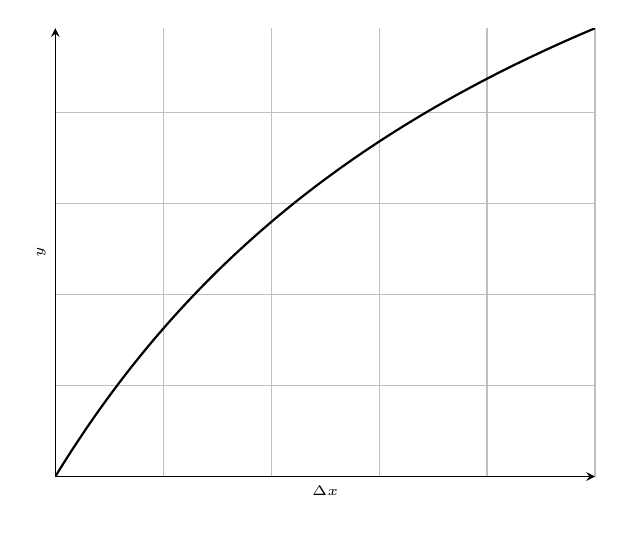
\begin{tikzpicture}[domain=0:4]
		\begin{axis}%
			[
				grid=major,
				ticks=none,
				xlabel={\tiny $\Delta x$},
				ylabel={\tiny $y$},
				axis x line=left,
				axis y line=left,
				no markers,
				domain=0:1000,
				restrict y to domain=0:1001
			]
			\addplot[thick,samples=400] (x,{1001 - 1001 * 1000/(1000 + 0.97 * x)});
			% \addplot[thick,samples=400,color=green] (x,{500 - 1000 * 500/(1000 + x)});
		\end{axis}
	\end{tikzpicture}
	\caption{\label{fig:swap-func} Зображення графіку функції обміну}
\end{figure}

Нехай існують дві різні пари обміну $X/Y$ із $f_{1}(x)$ та $f_{2}(x)$
відповідно:

\begin{equation*}
 \begin{aligned}
  f_{1}(x) = R_{Y} - \frac{R_{Y} R_{X}}{R_{X} + x\gamma} \\
  f_{2}(x) = R'_{Y} - \frac{R'_{Y} R'_{X}}{R'_{X} + x\gamma}
 \end{aligned}
\end{equation*}

де $R_{X}, R_{Y}$ та $R'_{X}, R'_{Y}$ --- це вклади (резерви) у першу та другу
пару відповідно. Розглянемо спільні точки двох функцій:

\begin{equation*}
  \begin{aligned}
	f_{1}(x) &= f_{2}(x) \\
	R_{Y} - \frac{R_{Y} R_{X}}{R_{X} + x\gamma} &=  R'_{Y} - \frac{R'_{Y} R'_{X}}{R'_{X} + x\gamma} \\
 \end{aligned}
\end{equation*}

Вивівши $x$ отримаємо такі корені:

\begin{equation*}
x_{1} = 0, x_{2} = \frac{R_{Y} R'_{X} - R'_{Y}R_{X}}{(R_{Y} - R'_{Y}) \gamma}
\end{equation*}

Звідси розглянемо три різні випадки:

\begin{enumerate}
  \item $R_{Y} \neq R'_{Y}$ та $R_{X} \neq R'_{X}$ --- криві мають точку перетину у
		$x_{2},x_{1}$ (рис.~\ref{fig:swap-funcs}).
  \item $R_{Y} = R'_{Y}$ та $R_{X} \neq R'_{X}$ --- криві мають перетин лише у
  $x = 0$.
  \item $R_{Y} = R'_{Y}$ та $R_{X} = R'_{X} \implies f_{1} = f_{2}$
\end{enumerate}

\begin{figure}[h!]
	\centering
	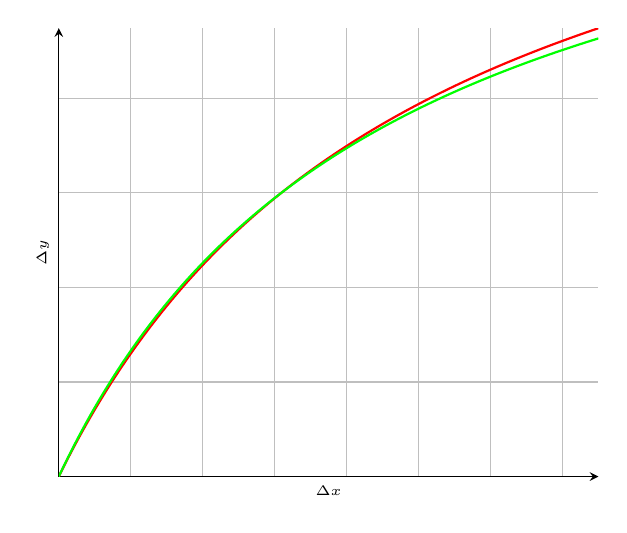
\begin{tikzpicture}[domain=0:4]
		\begin{axis}%
			[
				grid=major,
				ticks=none,
				xlabel={\tiny $\Delta x$},
				ylabel={\tiny $\Delta y$},
				axis x line=left,
				axis y line=left,
				no markers,
				domain=0:1500,
				restrict y to domain=0:1500
			]
			\addplot[thick,samples=400,color=red] (x,{1600 - 1600 * 1000/(1000 + 0.97 * x)});
			\addplot[thick,samples=400,color=green] (x,{1500 - 900 * 1500/(900 + 0.97 * x)});
		\end{axis}
	\end{tikzpicture}
	\caption{\label{fig:swap-funcs} Зображення графіку функцій обмінів при
	  $R_{Y} \neq R'_{Y}$ та $R_{X} \neq R'_{X}$ }
\end{figure}

У першому випадку існує така точка $x_{2}$ після котрої одна з кривих більша за
іншу, і до котрої меньша за іншу. Тобто об'єм результату обміну з $f_{1}$ стає
більшим за $f_{2}$ або навпаки. Достатньо легко перевірити яка саме через
нерівність:

\begin{equation*}
  f_{1}(x_{2} + \varepsilon) > f_{2}(x_{2} + \varepsilon)
\end{equation*}

\subsection{Композиція функцій обміну}\label{sec:func-composition}

Перед наступним розділом пропонуємо розглянути властивості та сутність
композицій функцій обміну. Нехай необхідно знайти об'єм обміну \(X \implies Y\),
з~\eqref{eq:swap-fee} це буде:

\begin{equation*}
	y = f_{X/Y}(x) = R_{Y} - \frac{R_{Y} R_{X}}{R_{X} + x \gamma}
\end{equation*}

Обмін \(Y \implies Z\):

\begin{equation*}
	z = f_{Y/Z}(y) = R_{Z} - \frac{R_{Z} R_{Y}}{R_{Y} + y \gamma}
\end{equation*}

Зафіксуємо об'єм $\Delta x$ валюти $X$ для отримання $\Delta y$ валюти $Y$:

\begin{equation}\label{eq:swap_xy}
	\Delta y = f_{X/Y}(\Delta x)
\end{equation}

І для наступного $\Delta y$ на $\Delta z$:

\begin{equation*}
	\Delta z = f_{Y/Z}(\Delta y)
\end{equation*}

З~\eqref{eq:swap_xy}:

\begin{equation*}
	\Delta z = f_{Y/Z}(\Delta y) = f_{Y/Z}(f_{X/Y}(\Delta x)) = (f_{X/Y} \circ f_{Y/Z})(\Delta x)
\end{equation*}

Звідси робимо висновок що композиція функція обміну, є аналогічним до обміну по
парам цих функцій.

\subsection{Об'єм отримуємий при \(n\)-тій кількості переходів.}\label{sec:nth-swap}

У кінцевій задачі ми будемо розглядати переходи між \(n\)-тою кількістю валют:

\begin{lemma} Нехай, \(R_{C_{i}}\) --- об'єм вкладів пари \textbf{на котру} ми
  вносимо валюту \(C_i\), а \(R_{C_{i+1}}\) --- об'єм вкладів пари \textbf{з
	котрої} ми виносимо валюту \(C_{i+1}\) при \(i\)-тому обміні, де
  \(i = \overline{0, n}\). Тоді об'єм обміну
  \(C_{0} \implies C_{1} \ldots \implies C_{n-1} \implies C_{n} \) при вхідному
  \(x\):

  \begin{equation}\label{eq:nth-swap}
	\begin{aligned}
	  y &= (f_{C_{0}/C_{1}} \circ f_{C_{1}/C_{2}} \circ \ldots f_{C_{i}/C_{i+1}})(x) = \\
	  &= x \prod_{i=1}^n R_{C_{i+1}} \div \left( \prod_{i=1}^{n} R_{C_{i}} + x \sum_{i=0}^{n-1} \left( \prod_{k=1}^i R_{C_{i+1}} \cdot \prod_{j=i+2}^{n}  R_{C_{i}} \right) \right)
	\end{aligned}
	\end{equation}
\end{lemma}

% Поки закометовано, бо не встиг довести.
% \begin{proof}
% Нехай, \(a_{X/Y}\) - кількість вкладів валюти \(X\) у пару \(X/Y\), \(b_{X/Y}\)
% -- кількість вкладів валюти \(Y\) у пару \(X/Y\), \(a_{Y/Z}\) - кількість
% вкладів валюти \(Y\) у пару \(Y/Z\), \(b_{Y/Z}\) - кількість вкладів валюти
% \(Z\) у пару \(Y/Z\).
%
% Тоді, з формули \eqref{eq:swap} ми можемо отримати кількість \(y\) валюти \(Y\) при
% вкладанні \(x\) валюти \(X\) у пару \(X/Y\):
%
% \begin{equation}
% y(x) = \frac{b_{X/Y}x}{(a_{X/Y} + x)}
% \end{equation}
%
% Розглянемо випадок коли \(y\) валюти \(Y\) вкладено у пару \(Y/Z\):
%
% \begin{equation*}
% z(y) = \frac{b_{Y/Z}y}{(a_{Y/Z} + y)}
% \end{equation*}
%
% Підставивши \(y(x)\) у \(z(y)\) отримаємо залежність \(z(x)\) від \(x\):
%
% \begin{equation*}
% \begin{aligned}
% z \circ y = z(y(x)) = \frac{b_{Y/Z}y(x)}{(a_{Y/Z} + y(x))} = \\
% \frac{b_{Y/Z} \frac{b_{X/Y}x}{(a_{X/Y} + x)}}{(a_{Y/Z} + \frac{b_{X/Y}x}{(a_{X/Y} + x)})} = \\
% \frac{b_{Y/Z}b_{X/Y}x}{(a_{X/Y} + x)(a_{Y/Z} + \frac{b_{X/Y}x}{(a_{X/Y} + x)})} = \\
% \frac{b_{X/Y}b_{Y/Z}x}{a_{X/Y} a_{Y/Z}  + (a_{Y/Z} + b_{X/Y}) x}
% \end{aligned}
% \end{equation*}
%
% Намагаючись знайти деяку закономірність, спробуємо розглянути ще один перехід
% \(Z \implies W\):
%
% \begin{equation*}
% w(z) = \frac{b_{Z/W}z}{(a_{Z/W} + z)}
% \end{equation*}
%
% Підставимо і його:
%
% \begin{equation*}
% \begin{aligned}
% w \circ z \circ y &= w(z(y(x))) = \frac{b_{Z/W}z(y(x))}{(a_{Z/W} + z(y(x)))} \\
% &= \frac{b_{Z/W} \frac{b_{X/Y}b_{Y/Z}x}{a_{X/Y} a_{Y/Z}  + (a_{Y/Z} + b_{X/Y}) x}}{(a_{Z/W} + \frac{b_{X/Y}b_{Y/Z}x}{a_{X/Y} a_{Y/Z}  + (a_{Y/Z} + b_{X/Y}) x})} \\
% &= \frac{b_{Z/W}b_{X/Y}b_{Y/Z}x}{a_{X/Y} a_{Y/Z} a_{Z/W} + (a_{Y/Z} a_{Z/W} + b_{X/Y} a_{Z/W} + b_{Y/Z} b_{X/Y}) x}
% \end{aligned}
% \end{equation*}
%
% Достатньо легко побачити, що у чисельнику утворюється добуток вкладів пари \textbf{на
% котру} ми обмінюємо, а у знаменику першим доданком добуток всіх вкладів \textbf{котрі}
% ми обмінюємо. Не очевидним залишається сума біля \(x\) у знаменику.
% \end{proof}

Так як $R_{C_{i}}$ є константами як і їх добуток та сума, зробивши заміну вигляду:

\begin{equation}\label{eq:swap-omega-xi}
\begin{aligned}
  R_{\Omega} &= \prod_{i=1}^n R_{C_{i+1}} \\
  R_{\Xi} &= \sum_{i=0}^{n-1} \left( \prod_{k=1}^i R_{C_{i+1}} \cdot \prod_{j=i+2}^{n}  R_{C_{i}} \right)
\end{aligned}
\end{equation}

Отримаємо функцію обміну:

\begin{equation*}
y = \frac{x R_{\Omega}}{R_{\Omega} + x R_{\Xi}}
\end{equation*}

Таким чином, рівняння~\eqref{eq:nth-swap} зберігає всі властивості функції
обміну.

Результат дозволяє в один математичний вираз описати декілька переходів, проте
при обрахуванні методами програмного забезпечення добутки вкладів можуть бути
настільки великими числами (навіть два обміни між парами із вкладами по \(10^6\)
утворює числа \({(10^6)}^3\)), що при використанні чисел із обмеженою точністю
можуть утворювати переповнення.

На момент написання цієї роботи, максимальний розмір регістра
середньостатистичного комерційного комп'ютера скаладав 64 біта, де максимальне
значення числа без знаку становить \(2^{64} < 10^{20}\).
\end{document}
